\documentclass[11pt]{article}

\usepackage[margin=1.2in, a4paper]{geometry}

\usepackage[utf8]{inputenc}

\usepackage{setspace}  % set spacing

\setstretch{1.25}  %stretch line space to multiple x

\usepackage[dvipsnames,table, xcdraw]{xcolor}
% If you use beamer only pass "xcolor=table" option, i.e. \documentclass[xcolor=table]{beamer}

\usepackage{shadowtext}

\usepackage{indentfirst} % indent the first paragraph of each section

\usepackage{float} %determine the position of figures in the document

\usepackage{tabularx} % extra features for tabular environment

\usepackage{amsmath, amsfonts, amssymb}  % improve math presentation

\usepackage{blkarray, bigstrut}

\usepackage{makecell}

\usepackage{mathtools}
\DeclarePairedDelimiter\ceil{\lceil}{\rceil}
\DeclarePairedDelimiter\floor{\lfloor}{\rfloor}



%++++++++++++++++++++++++++++++++++++++++++++++++++++++++++++++++

\usepackage{graphicx} % takes care of graphic including machinery

\graphicspath{{images/}}

%++++++++++++++++++++++++++++++++++++++++++++++++++++++++++++++++



\usepackage{caption}

\usepackage{subcaption}

\usepackage{tikz}

\usepackage{lipsum,lmodern}

\usepackage[most]{tcolorbox}

\usetikzlibrary{trees}  %add binary trees

\usetikzlibrary {positioning}

\usepackage[final]{hyperref} % adds hyper links inside the generated pdf file

\hypersetup{
	colorlinks=true,       % false: boxed links; true: colored links
	linkcolor=blue,        % color of internal links
	citecolor=blue,        % color of links to bibliography
	filecolor=magenta,     % color of file links
	urlcolor=blue         
}

\usepackage{blindtext}

\usepackage{dirtytalk} %quotation marks


%********************************

%Bibliography

\usepackage[backend=biber,  style=alphabetic,  sorting=ynt]{biblatex}

\addbibresource{../../Mybib.bib}


%********************************


\usepackage{fancyhdr}

\pagestyle{fancy}

\fancyhf{}

\lhead{\footnotesize {Mathematical Statistics} }
\rhead{\footnotesize { } }
\cfoot{- \thepage \ -}

\title{\vspace{-90pt} 


%**************************************************

% Title Part
\textbf  {Peer-graded Assignment} }
\author{Cui, Xiaolong(Larry)}
\date{\today}


%*************************************************

\begin{document}

%\maketitle

\thispagestyle{plain}

%*************************************************

\begin{figure}[H] %[!tbp]
  \begin{subfigure}{0.3\textwidth}
    
\includegraphics[width=\textwidth]{uol}
    %\caption{Flower one.}
    %\label{fig:f1}
  \end{subfigure}
  \hfill
  \begin{subfigure}{0.3\textwidth}
    \includegraphics[width=\textwidth]{goldsmiths}
    %\caption{Flower two.}
    %\label{fig:f2}
  \end{subfigure}
  %\caption{My flowers.}
\end{figure}

%****************************************************

\begin{flushright}

\footnotesize {July 04 2021}
\end{flushright}

\begin{center}
\textbf{Stirling's Formula to De Moivre \& Laplace Theorem} \\
\footnotesize {Study Notes $ | $ Written by Larry Cui}
\end{center}

%***************************************************

\begin{abstract}
Stirling formula and De Moivre Laplace theorem are important intermediate steps toward the central limit theorem.  However,  in some undergraduate textbooks on mathematical statistics,  the step by step proof is usually omitted,  which I found sometimes poses quite a huge challenge for students to fully understand the logic behind the formula of normal distribution.  This is the reason I digged into the internet for helps.  Among numerous articles and papers, I referred frequently to \cite{balazs2014stirling} and Jacek Cichon's "Stirling Approximation Formula" for my note,  and appreciate a lot for their generous share of knowledges.
\end{abstract}


%***************************************************

\setcounter{figure}{0}

\vspace{10pt}


\section {\large Stirling's Formula}


Stirling's formula is used during the proof of De Moivre Laplace Theorem.  It's an approximation of the n factorial,  which takes the following form:

\begin{tcolorbox} 
[colback=blue!5!white,  colframe=blue!75!black,  title= {\textbf{
Stirling's Formula
} }]

$$ n! \approx \sqrt{ 2 \pi n} \left(  \frac{n}{e} \right) ^n $$

\end{tcolorbox}


\section {\large A rough Estimate}

If we take  logarithm of $n!$,  the product of \say {$1 \cdot 2 \cdot 3 \cdots n$} becomes the sum of logarithms (let's name it as \say { $S(n)$ } ),  i.e.,  $ S(n) = \ln 1 + \ln 2 + \cdots + \ln n$.   Now we can use some comparisons as shown below:

\begin{figure}[H] 
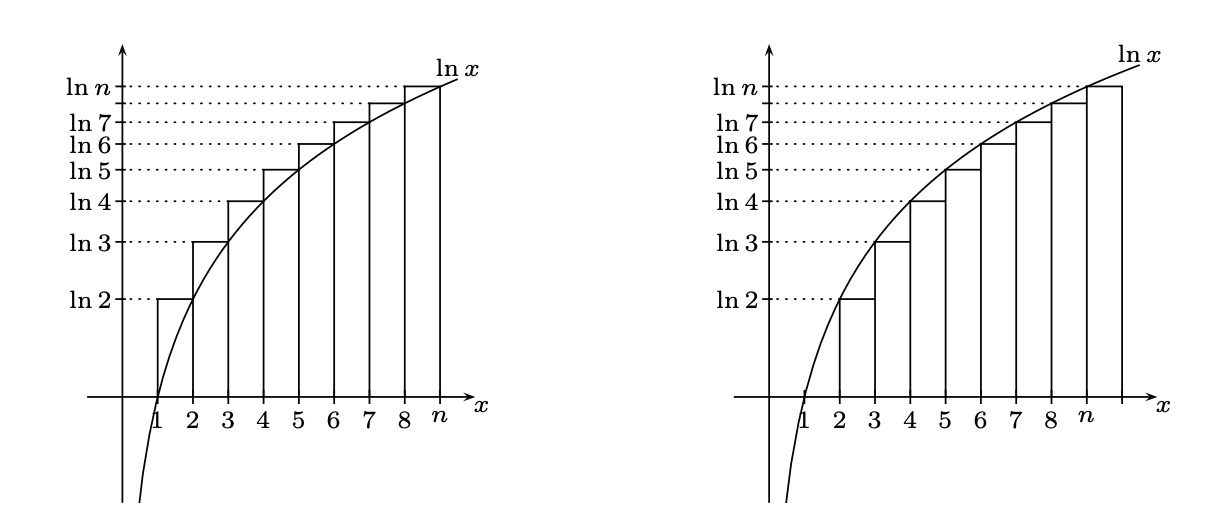
\includegraphics [scale = 0.6] {comparison} %[width=\textwidth]
\centering
\caption{$S(n)$ vs.  $\ln x$ }
\label{fig:f1}
\end{figure}

We can directly derive the following bounds:

\begin{equation}
 \int^{n}_{1} \ln x dx \leqslant  S(n) \leqslant \int ^{n+1} _ {1} \ln x dx
\end{equation}


Integrate the left side of the above formula,  we have $ \displaystyle  \int ^n _1 \ln x dx = (x \ln x - x) \bigg \rvert ^n _1 = n \ln n -n - 1* \ln 1 + 1 = n \ln n - (n - 1) $.  The same integrated form is used to get the result for $ \displaystyle \int ^{n+1} _ {1} \ln x dx =  (n+1) \ln (n+1) - n $.  

We now can change the formula into the form
\begin{equation}
 \ln \frac {n^n}{e^{n-1}} \leqslant S(n) \leqslant \ln \frac{(n+1)^{n+1}}{e^n}
\end{equation}

Since $n! = \exp [S(n)]$,  we get the esp. (1) in the form

\begin{equation}
\frac {n^n}{e^{n-1}} \leqslant n! \leqslant  \frac{(n+1)^{n+1}}{e^n}
\end{equation} 

Becasue $\displaystyle \frac{(n+1)^{n+1}}{e^n} = \left( \frac{n+1}{e} \right) ^n  (n+1) = \left( \frac{n}{e} \cdot \frac{n+1}{n} \right) ^n (n+1) = \left( \frac{n}{e} \right) ^n \cdot \left( 1 + \frac{1}{n} \right) ^n (n+1) $,  and as $n \to \infty$,  $\displaystyle \left( 1 + \frac{1}{n} \right) ^n = e$,  the right side of esp. (3) becomes $ \displaystyle e(n+1) \left( \frac{n}{e} \right) ^n$,  we have a neater form of eq. (3) as
$$ e \left( \frac{n}{e} \right) ^n \leqslant n! \leqslant e(n+1) \left( \frac{n}{e} \right) ^n $$
which is saying that 
\begin{equation}
n! = f(n) \left( \frac{n}{e} \right) ^n
\end{equation}
for a function $f(n)$ where $ e \leqslant f(n) \leqslant e(n+1) $.


\section {\large Finding Constant C}

We re-arrange eq. (4) by dividing both sides with $ \displaystyle \sqrt{2n} \left( \frac{n}{e} \right) ^n $,  we have 
$$ \displaystyle  \frac {n!}  { \sqrt{2n}  \left( \frac{n}{e} \right) ^n } = \frac {f(n)} { \sqrt{2n} } $$
Why we need to divide with $ \sqrt {2n}$ cannot be deduced from the equation itself,  but let's assume for the time being that $ \displaystyle  \frac {n!}  { \sqrt{2n}  \left( \frac{n}{e} \right) ^n } $ approaches to some constant number $C$,  and we are going to find this number so that $\displaystyle n! \approx C  \sqrt{2n}  \left( \frac{n}{e} \right) ^n $.


\subsection{\normalsize The integration of $ \displaystyle \int \sin ^n x dx$}

Integrating by parts we get
$$
\begin{aligned}[t]
\int \sin ^n x dx
    &= \int \sin ^{n-1} x \sin x dx\\
    &= - \sin ^{n-1} x \cos x + \int (n-1) \sin ^{n-2} x \cos ^2 x dx \\
    &= - \sin ^{n-1} x \cos x + \int (n-1) \sin ^{n-2} x (1 - \sin ^2 x)  dx \\
    &= - \sin ^{n-1} x \cos x + \int (n-1) \sin ^{n-2} x dx -  \int (n-1)  \sin ^n x  dx \\
n \int \sin ^n x dx &= - \sin ^{n-1} x \cos x + (n-1) \int \sin ^{n-2} x dx \\
\end{aligned}\\
$$
so
$$
\begin{aligned}[t]
\int \sin ^n x dx 
	&= - \frac{1}{n} \sin ^{n-1} x \cos x + \frac{n-1}{n} \int \sin ^{n-2} x dx \\
\end{aligned}\\
$$
If we evaluate from $\displaystyle 0 \sim \frac{\pi}{2}$,  the above equation reduces to
$$ \int _0 ^{\pi/2} \sin ^n x dx = \frac{n-1}{n} \int _0 ^{\pi/2} \sin ^{n-2} x dx $$
(a) for $\displaystyle n=2k,  S_{even} = \int _0 ^{\pi /2} \sin ^{2k} x dx = \frac{2k-1}{2k} \cdot \frac{2k-3}{2k-2} \cdots \frac{1}{2} \cdot \int _0 ^{\pi/2} \sin ^0 x dx $,  we have
\begin{equation}
S_{even} = \frac{\pi}{2} \prod _{k=1} ^{n/2} \frac{2k-1}{2k}
\end{equation}
(b) for $\displaystyle n=2k+1,  S_{odd} = \int _0 ^{\pi /2} \sin ^{2k+1} x dx = \frac{2k}{2k+1} \cdot \frac{2k-2}{2k-1} \cdots \frac{2}{3} \cdot \int _0 ^{\pi/2} \sin ^1 x dx \\
=  \prod _{k=1} ^{(n-1)/2} \frac{2k}{2k+1} \cdot (-\cos x) \bigg \rvert _0 ^{\pi/2} $, we have

\begin{equation}
S_{odd} = \prod _{k=1} ^{(n-1)/2} \frac{2k}{2k+1}
\end{equation}


\subsection{\normalsize Wallis product formula}

\begin{tcolorbox} 
[colback=blue!5!white,  colframe=blue!75!black,  title= {\textbf{
Wallis Formula
} }]

$$ \prod _{n=1} ^{\infty } \frac{2n}{2n-1} \frac {2n}{2n+1} = \frac{\pi}{2} $$

\end{tcolorbox}

From eq. (5) and (6),  we can tell that when $k$ and $n$ goes to $\infty$,  the left side of Wallis formula is actually $\displaystyle \frac{\pi}{2} \cdot \frac {S_{odd}}{S_{even}}$ and for $x \in (0,  \pi/2)$,  
$$ 0 < \sin ^{2k+2} x < \sin ^{2k+1} x < \sin ^{2k} x $$
and $$ 0 < S_{2k+2} < S_{2k+1} < S_{2k} $$
divide by $S_{2k}$ on each term,  we have 
$$ 0 < \frac{S_{2k+2}}{S_{2k}} < \frac{ S_{2k+1} } {S_ {2k}} < 1 $$
Because $\displaystyle \lim _{k \to \infty} \frac{S_{2k+2}}{S_{2k}} = \lim _{k \to \infty} \frac{2k+1}{2k+2} = 1  < \frac{S_{2k+1}}{S_{2k}} < 1 $,  according to squeeze theorem,  $ \displaystyle  \frac{S_{2k+1}}{S_{2k}} =  1 $.  This proves the Wallis formula.  \\

Now we can use Wallis formula to obtain constant $C$,  but first of all,  we need to re-write the Wallis formula in a compact way:
$$
\begin{aligned}[t]
 \prod _{n=1} ^{n } \frac{2n}{2n-1} \frac {2n}{2n+1}
    &= 2^{2n} (n!)^2  \prod _{n=1} ^{n } \frac{1}{2n-1} \frac{1}{2n+1}\\
    &= 2^{2n} (n!)^2 \cdot \frac{2 \cdot 4 \cdots 2n}{(2n)!} \cdot \frac{2 \cdot 4 \cdots 2n}{(2n+1)!}\\
    &= \frac{2^{2n} (n!)^2 2^{2n} (n!)^2} {((2n)!)^2 (2n+1)}\\
\end{aligned}\\
$$
so
\begin{equation}
 \prod _{n=1} ^{n } \frac{2n}{2n-1} \frac {2n}{2n+1} = \frac{2^{4n} (n!)^4} {((2n)!)^2 (2n+1)}
\end{equation}
since we pick $C$ so $\displaystyle n! \approx C  \sqrt{2n}  \left( \frac{n}{e} \right) ^n $,  and the formula still holds if we substitute $n$ by $2n$:  $\displaystyle (2n)! \approx C  \sqrt{4n}  \left( \frac{2n}{e} \right) ^{2n} $,  we can replace $n!$ and $(2n)!$ with $C$ formula into eq. (7)
$$
\begin{aligned}[t]
\frac{2^{4n} (n!)^4} {((2n)!)^2 (2n+1)}
	&= \frac{2^{4n} (C  \sqrt{2n}  \left( \frac{n}{e} \right) ^n ) ^4 } { (C \sqrt{4n} ( \frac{2n}{e} ) ^{2n} ) ^2 (2n+1)} \\
	&= \frac{2^{4n} C^4  4n^2  \left( \frac{n}{e} \right) ^{4n} } { C^2 4n ( \frac{2n}{e} ) ^{4n} (2n+1)} \\
	&= \frac{2^{4n} C^2  n  \left( \frac{1}{2} \right) ^{4n} } { 2n+1} \\
	&= C^2 \frac{n} {2n+1} \\
\end{aligned}\\
$$
from Wallis formula,  we know
$$ \lim _{n \to \infty}  C^2 \frac{n} {2n+1} = \frac{\pi}{2} $$
so the C for Stirling approximation: $$C = \sqrt{\pi}$$


\section{\large Proof of the Existence of the Limit and the Error Boundary}

Although we've found constant $C = \sqrt{\pi}$,  we haven't proved $\displaystyle  \sqrt{2n \pi}  \left( \frac{n}{e} \right) ^n $ stays within what interval of the exact number $n!$.  Now let's take a second look as eq. (3),  we can re-write the formula as
$$ n \ln n - n + 1 \leqslant \ln n! \leqslant (n+1) \ln (n+1) - n $$
true as well is the following formula
$$  n \ln n - n  \leqslant \ln n! \leqslant (n+1) \ln (n+1) - n $$


We've already had the approximation of $\ln n!$ when $n \to \infty$ in Section 3,  but we don't know how good the approximation is.   Now we arbitrarily pick a number between $n \ln n - n$ and $(n+1) \ln (n+1) - n$,  for example,  $(n + \frac{1}{2}) \ln n - n$,  and look at the difference (maybe not arbitrarily picked,  for this number and the difference formed by it helps reach the conclusion below): 
$$ d_n = \ln n! - \left[(n + \frac{1}{2}) \ln n - n \right] $$
We don't know if $\ln n!$ is greater than $[(n + \frac{1}{2}) \ln n - n ] $ or not,  but the result won't be different as we are looking into the tendency of $d_n$.  We want to prove the following two properties:

(a) $d_n $ is monotone decreasing and converges to a limit $d$,  as we've already find the approximation for $\ln n!$,  here $\displaystyle \lim _{n \to \infty } d = \ln \sqrt{2 \pi n}  \left( \frac{n}{e} \right) ^n -\left[ \left(n + \frac{1}{2} \right) \ln - n \right] $;

(b) for every $n$,  we have $d < d_n < d + \frac{1}{12n}$.\\

\subsection{\normalsize Monotone Decreasing of $d_n$ toward $d$}

If we look at the decrement of $d_n$:
$$
\begin{aligned}[t]
d_n - d_{n+1}
    &=  \ln n! - \left[(n + \frac{1}{2}) \ln n - n \right]  -  \ln (n+1)! + \left[(n + \frac{3}{2}) \ln (n+1) - n - 1 \right] \\
    &= - \ln (n+1)-  (n + \frac{1}{2}) \ln n + n +  (n + \frac{3}{2}) \ln (n+1) - n - 1  \\
    &= (n + \frac{1}{2}) \ln \frac{n+1}{n} - 1  \\
\end{aligned}\\
$$
Now we need some techniques from Taylor Series expansion.  First of all,  we use $t= \displaystyle  \frac{1}{2n+1}$ to re-write the above formula as
$$ \frac{1}{2t} \ln \frac{1+t}{1-t} -1 $$
then we use polynomial to express the form of $\ln (1+t)$:
$$ \ln (1+t) = t - \frac{t^2}{2} + \frac{t^3}{3} - \cdots =  - \sum _{k=1} ^\infty (-1)^k \frac{t^k}{k} $$
and the form of $\ln (1-t)$:
$$ \ln (1-t) = -t -  \frac{t^2}{2} - \frac{t^3}{3} - \cdots = - \sum _{k=1} ^\infty \frac{t^k}{k} $$
so
\begin{equation}
\begin{aligned}[b]
 d_n - d_{n+1} 
 	&= \frac{1}{2t} \left(  - \sum _{k=1} ^\infty (-1)^k \frac{t^k}{k} +  \sum _{k=1} ^\infty \frac{t^k}{k} \right) -1 \\
 	&= \frac{1}{2t} \sum _{k=0} ^\infty \frac{2t^{2k+1}} {2k+1}  -1 \\
	&=  \frac{1}{t} \sum _{k=1} ^\infty \frac{t^{2k+1}} {2k+1} 
\end{aligned}
\end{equation}


as $n \to \infty$,  $t \to 0$ from the positive side,  so always $ d_n - d_{n+1} \geqslant 0 $,  and $d_n$ is monotone decreasing. \\


\subsection{\normalsize $d$ bounded below by $b_n - 1/12n$}

Proceed with eq. (8), 
$$
\begin{aligned}[b]
 d_n - d_{n+1} =  \frac{1}{t} \sum _{k=1} ^\infty \frac{t^{2k+1}} {2k+1} < \sum _{k=1} ^\infty \frac{t^{2k}} {3} 
 	&= \frac{1}{3} \cdot \frac{t^2}{1- t^2} \\
	&= \frac{1}{3} \cdot \frac{1}{(2n+1)^2 -1}  & (\text{remark:} \ \  t=\frac{1}{2n+1}) \\
	&= \frac{1}{12} \cdot \frac{1}{n^2 + n} \\
	&= \frac{1}{12} \cdot \frac{1}{n} - \frac{1}{12} \cdot \frac{1}{n+1}\\
\end{aligned}
$$
re-arrange it,  we have
$$
 d_n - \frac{1}{12} \cdot \frac{1}{n}  < d_{n+1} - \frac{1}{12} \cdot \frac{1}{n+1} 
$$
which means function $ \displaystyle \left( d_n - \frac{1}{12} \cdot \frac{1}{n} \right) $ is increasing.  In short,  we prove that limit $d \in (d_n - 1/12n, d_n)$,  and we have the following inequality:
\begin{equation}
d < d_n < d + \frac{1}{12n} 
\end{equation}


\subsection{\normalsize the Error Boundary}

Let $\displaystyle g(n) = \ln  \sqrt{2 \pi n}  \left( \frac{n}{e} \right) ^n$ for short,  eq. (9) becomes
$$
g(n) - \left[ \left(n + \frac{1}{2} \right) \ln n - n \right] <  \ln n! - \left[ \left(n + \frac{1}{2} \right) \ln n - n \right] < g(n) - \left[ \left(n + \frac{1}{2} \right) \ln n - n \right] + \frac{1}{12n}
$$
take them to the power of $\mathsf{e}$,  we have the boundary below
$$
\begin{aligned}[b]
\frac{e ^ {g(n) + n } }{n ^ {n + 1/2} } &< \frac{n! \cdot e^n}{n ^ {n + 1/2} } < \frac{e ^ {g(n) + n + 1/12n} }{n ^ {n + 1/2} }  \\
1 &< \frac{n!}{e^{g(n)} } < e ^{1/12n} \\
\sqrt{2 \pi n}  \left( \frac{n}{e} \right) ^n &< n! <  \sqrt{2 \pi n}  \left( \frac{n}{e} \right) ^n \left(1+ e ^{1/12n} \right) \\
\end{aligned}
$$




%++++++++++++++++++++++++++++++++++++++++


\printbibliography [title={Reference}]


%***********************************

\end{document}
